\documentclass{standalone}

\usepackage{tikz}
\usepackage{amssymb}
\usetikzlibrary{trees}

\begin{document}
	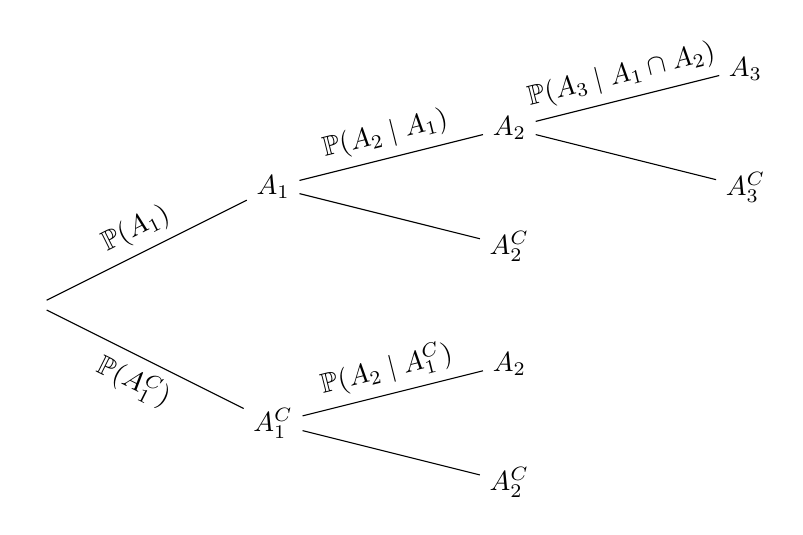
\begin{tikzpicture}[level distance=3cm,
	level 1/.style={sibling distance=3cm},
	level 2/.style={sibling distance=1.5cm},
	grow=right, sloped]
	\node {}
	child {node {$A_1^C$}
		child {node {$A_2^C$}}
		child {node {$A_2$} edge from parent node[above]  {$\mathbb{P}(A_2\mid A_1^C)$}}
		edge from parent
		node[below]  {$\mathbb{P}(A_1^C)$}
	}
	child {node {$A_1$}
		child {node {$A_2^C$}}
		child {node {$A_2$}
			child {node {$A_3^C$}}
			child {node {$A_3$} edge from parent node[above]  {$\mathbb{P}(A_3\mid A_1\cap A_2)$}}
			edge from parent
			node[above]  {$\mathbb{P}(A_2\mid A_1)$}}
		edge from parent
		node[above]  {$\mathbb{P}(A_1)$}
	};
	\end{tikzpicture}
\end{document}
